\documentclass[12pt]{beamer}
\usepackage[T2A]{fontenc}
\usepackage[utf8]{inputenc}
\usepackage[english,russian]{babel}
\usepackage{amssymb,amsfonts,amsmath,mathtext}
\usepackage{cite,enumerate,float,indentfirst}

\graphicspath{{images/}}

\usetheme{Singapore}
%\usecolortheme{whale}

\setbeamertemplate{navigation symbols}{} %remove navigation symbols at all
\setbeamercolor{footline}{fg=black}
\setbeamerfont{footline}{size=\fontsize{8}{10}\selectfont}
\setbeamersize{text margin left=0.6cm, text margin right=0.4cm}
\setbeamertemplate{footline}{
  \leavevmode%
  \hbox{%
    \begin{beamercolorbox}[wd=.5\paperwidth,ht=2.5ex,dp=1ex,left]{}%
      Я. А. Воронцов, ВГУ
    \end{beamercolorbox}%
    \begin{beamercolorbox}[wd=.5\paperwidth,ht=2.5ex,dp=1ex,right]{}%
      \insertframenumber{} / \inserttotalframenumber \hspace*{2ex}
    \end{beamercolorbox}
  }%
  \vskip0pt%
}

\newcommand{\itemi}{\item[\checkmark]}

\title{\Large{Модели и методы решения задач с нечеткими параметрами и четкими отношениями}}
\author{\normalsize{%
Я. А. Воронцов\\%
\emph{Научный руководитель:}~М.Г.Матвеев,~д.т.н.,~профессор.}\\%
\small{
\vspace{10pt}
Материалы для защиты диссертации на соискание учёной степени кандидата физико-математических наук \\
Специальность 05.13.18~--- математическое моделирование,\\ численные методы и комплексы программ \\
\vspace{10pt}
ФГБОУ ВПО <<Воронежский государственный университет>>%
\vspace{10pt}%
}
\small{Воронеж, 2015}
}

\begin{document}

\maketitle

\begin{frame}
  \frametitle{Цель и задачи исследования}
  \textbf{Цель:} построение и исследование моделей учёта нечёткой неопределённости, обеспечивающих требуемые свойства решения различных прикладных задач, а также разработка методов эффективного численного решения на основе вводимых моделей \\
  \textbf{Задачи:}
  \begin{itemize}
    \item анализ существующих методик нечётких вычислений с~точки зрения сохранения свойств решения задач;
    \item разработка модели представления нечётких чисел, позволяющей максимально сохранять исходную экспертную информацию и обеспечить требуемые качественные свойства решений (устойчивость, сохранение чётких математических соотношений и т.\,п.);
  \end{itemize}  
\end{frame}

\begin{frame}
  \frametitle{Цель и задачи исследования}
  \begin{itemize}
    \item разработка методики эффективной численной реализации решения задач с нечёткими параметрами, основанной на подходящих алгебраических структурах и её тестирование на примере задачи сетевого планирования с нечёткими параметрами;
    \item разработка и верификация программного обеспечения, реализущего предложенную модель представления нечётких параметров и методики численного решения задач с нечёткими параметрами.
  \end{itemize}  
\end{frame}


\begin{frame}
  \frametitle{Научная новизна}
  \begin{itemize}
    \item \textbf{модификация метода моделирования экспертных числовых оценок}, полученных в классе LR-чисел, отличающаяся наличием L-преобразования LR-числа в соответствующие LL/RR-числа;
    \item \textbf{эффективные вычислительные методы решения задач с нечёткими параметрами}, отличающиеся использованием описанной в работе алгебраической структуры (поле модифицированных нечётких чисел) и позволяющие параметрически управлять устойчивостью решения;
    \item \textbf{программный комплекс} для решения задачи сетевого планирования с нечёткими параметрами, реализующий предложенные вычислительные методы, модули которого используют стандартные вычислительные операции (в отличие от специализированных программных пакетов).
  \end{itemize}
\end{frame}

\begin{frame}
  \frametitle{Представление нечёткой информации}
  \begin{itemize}
    \item нечёткие множества (подмножества предопределённого универсального множества X)
      \begin{equation}
      	\tilde{A}=\left\{ \left( x, \mu_{\tilde A}\left( x \right) \right)\left| x\in X \right. \right\};\ E \left( \mu_{\tilde A} \left( x \right) \right) = \left[0; 1 \right]
      \end{equation}      
    \item нечёткие числа (подмножества множества действительных чисел $\mathbb{R}$)
      \begin{itemize}
        \item кусочная непрерывность $\mu_{\tilde A}\left( x \right)$;
        \item выпуклость $\mu_{\tilde A}\left( x \right)$
      	\begin{gather}
      	  \forall x_1, x_2 \in \mathbb{R}; \forall \gamma \in \left[ 0;1 \right] \notag \\
      	  \mu_{\tilde A}\left( \gamma x_1+\left( 1-\gamma  \right)x_2 \right)\geqslant \min \left\{ \mu_{\tilde A}\left( x_1 \right),\mu_{\tilde A}\left( x_2 \right) \right\}
      	\end{gather}
      	\item нормальность $\mu_{\tilde A}\left( x \right)$
        	\begin{equation}
        		\underset{x\in \mathbb{R}}{\mathop {\sup}}{}\, \left( \mu_{\tilde A} \left( x \right) \right)=1
        	\end{equation}
      \end{itemize}
  \end{itemize}
\end{frame}

\begin{frame}
  \frametitle{Классификация нечётких моделей}
  \begin{columns}[onlytextwidth]
    \begin{column}{0.6\textwidth}
      \begin{figure}[h]
        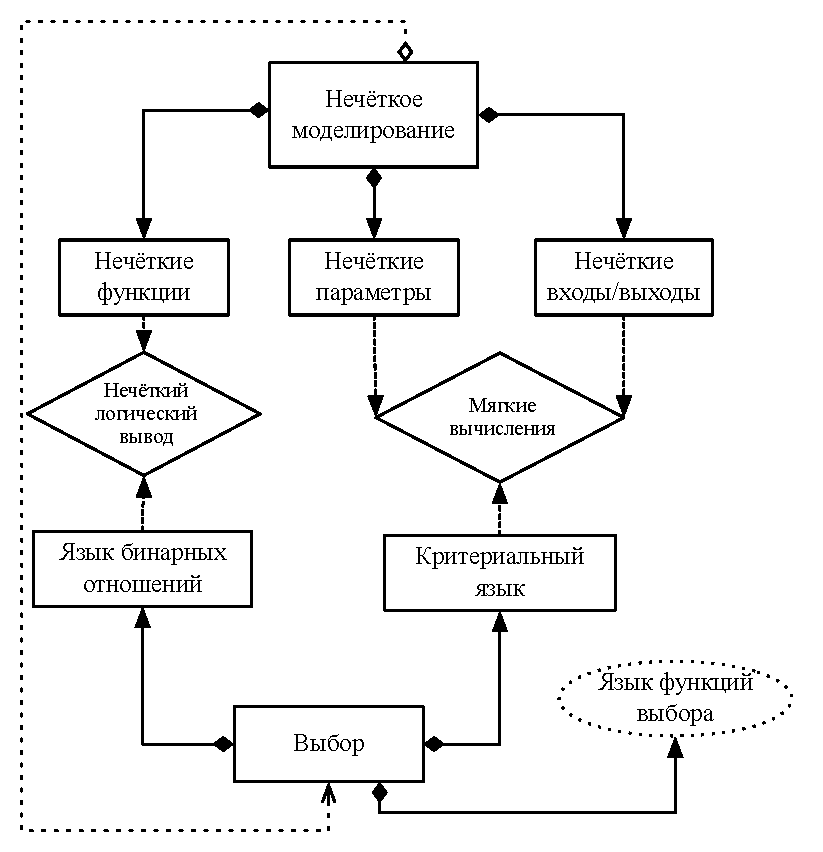
\includegraphics[width=\textwidth]{choice-classification}
      \end{figure}
    \end{column}
    \begin{column}{0.4\textwidth}
      \begin{itemize}
        \item Исследуются модели, использующие чёткие отношения и нечёткие параметры (модели второго типа)
        \item Существующие подходы к нечётким вычислениям далеко не всегда применимы в моделях второго типа
      \end{itemize}
    \end{column}
  \end{columns}
\end{frame}

\begin{frame}
  \frametitle{Проблемы существующих способов вычислений}
  \begin{itemize}
    \item 123
    \item 456
  \end{itemize}
\end{frame}

\begin{frame}
  \frametitle{Требования к разрабатываемой методике}
  \begin{itemize}
	\item ограничение роста неопределенности результатов обработки нечеткой информации;
	\item сохранение чётких отношений в модельных уравнениях при подстановке данных;
	\item возможность представления линейного порядка на множестве нечётких чисел;
	\item возможность использования стандартных программных средств реализации численных методов решений;
	\item возможность управления устойчивостью решения решаемой задачи.
  \end{itemize}
\end{frame}

\begin{frame}
  \frametitle{Основные понятия}
  \begin{itemize}
    \item 
  \end{itemize}

  \begin{equation}
    \label{eq:membership-alphacut-form}
	\left[ 
		\begin{aligned}
			& x^L(\alpha )=m-a+a\alpha  \\ 
			& x^R(\alpha )=m+b-b\alpha
		 \end{aligned}
	\right.
  \end{equation}
\end{frame}

\begin{frame}
  \frametitle{Основные понятия}
  \begin{itemize}
    \item Теорема о декомпозиции 
      \begin{equation}
        \tilde{A}=\bigcup\limits_{\alpha \in \left[ 0;1 \right]}{A_\alpha}
      \end{equation}
  \end{itemize}
\end{frame}


\begin{frame}
  \frametitle{Основные понятия}
    
\end{frame}

\begin{frame}
  \frametitle{Преобразование L}
  Исходная задача $\tilde{Y}=f\left( \tilde{X}, \tilde A \right)$ с нечёткими числовыми параметрами и~переменными рассматривается как совокупность задач с интервальной неопределенностью
  \begin{equation}
  \label{eq:alpha-equivalence}
  	\tilde{Y} = f\left( \tilde X, \tilde A \right)\to \bigcup\limits_{\alpha =0}^{1}{y_\alpha}=f\left( X_\alpha, A_\alpha \right)
  \end{equation}
  с последующим переходом к полной определённости на каждом $\alpha$-уровне, для чего на каждом $\alpha$-уровне внутри интервала $X_\alpha$ выбирается точка $\bar{x}\left( \alpha  \right)$. Предлагается выбирать значение $\bar{x}\left( \alpha  \right)$ с~помощью линейного параметрического преобразования $L$
  \begin{equation}
    \label{eq:L-transform-base}
    \bar{x}\left( \alpha  \right)=L\left( X_\alpha \right)=\lambda x^L \left( \alpha  \right)+\left( 1-\lambda  \right) x^R \left( \alpha  \right).
  \end{equation}
\end{frame}

\begin{frame}
  \frametitle{Модифицированные нечёткие числа}
  
\end{frame}

\begin{frame}
  \frametitle{Свойства преобразования L}
\end{frame}

\begin{frame}
  \frametitle{Алгебра модифицированных нечётких чисел}
\end{frame}

\begin{frame}
  \frametitle{Двухточечные вычисления}
\end{frame}

\begin{frame}
  \frametitle{Устойчивость задачи ЛП}
\end{frame}

\begin{frame}
  \frametitle{Устойчивость задачи ЛП}
\end{frame}

\begin{frame}
  \frametitle{Задача сетевого планирования}
\end{frame}

\begin{frame}
  \frametitle{Модифицированная задача сетевого планирования}
\end{frame}

\begin{frame}
  \frametitle{Решение задачи сетевого планирования}
\end{frame}

\begin{frame}
  \frametitle{Результат решения задачи}
\end{frame}

\begin{frame}
  \frametitle{Программное обеспечение}
\end{frame}

\begin{frame}
  \frametitle{Главное окно приложения}
  \begin{figure}
    \center
    \includegraphics[width=0.9\textwidth]{app-sample-graph.png}
  \end{figure}
\end{frame}

%\begin{frame}
%\frametitle{Таблица}
%\begin{tabular}{|l|l|}
%\hline
%\textbf{Заголовок 1} & \textbf{Заголовок 2} \\
%\hline
%Сумма & $b+a$ \\
%\hline
%Разность & $a-b$ \\
%\hline
%Произведение & $a*b$ \\
%\hline
%\end{tabular}
%\end{frame}


%%%%%%%%%%%%%%%%%%%%%%%%%%%%%%

\begin{frame}
  \frametitle{Результаты работы}
  \begin{itemize}
    \item Комплекс методов для моделей с чёткими отношениями и нечёткими параметрами
    \begin{itemize}
      \item применение классических методы решения
      \item достижение требуемых качественных свойств решения
    \end{itemize}
    \item Параметрическая модель представления нечёткого числа
    \begin{itemize}
      \item максимальное сохранение экспертной информации
      \item двухточечные вычисления~--- эффективная численная реализации решения
    \end{itemize}
    \item Устойчивость решения задачи линейного программирования с нечёткими параметрами
    \begin{itemize}
      \item свёртка критериев для управления устойчивостью
      \item алгоритм получения устойчивого решения задачи
    \end{itemize}
    \item Апробация методов~--- задача сетевого планирования
    \item Программный комплекс~--- решение задачи оценки сроков разработки программного обеспечения
  \end{itemize}
\end{frame}

\begin{frame}
  \frametitle{Апробация работы и публикации}
  Основные положения работы докладывались на конференциях:
  \begin{itemize}
    \item Современные проблемы прикладной математики, теории управления и математического моделирования (Воронеж, 2012 г.)
    \item Информатика: проблемы, методология, технологии (Воронеж, 2013--2014 гг.);
    \item Современные технологии в задачах управления, автоматики и обработки информации (Алушта, 2013--2014 гг.);
    \item Радиоэлектроника, электротехника и энергетика (Москва, 2014).
  \end{itemize}
  Основное содержание диссертационного исследования изложено в 11 научных работах, из~них 4 статьи в~изданиях, рекомендованных ВАК РФ.
\end{frame}

\end{document} 